\documentclass{beamer}
\usepackage{wasysym}
\usepackage{proof}
\usepackage{cancel}
\usepackage{chronology}
\usepackage{graphicx}
\usepackage{ulem}
\usepackage{amsmath}
\usepackage{amssymb}
\usepackage{color}
\usepackage{xcolor}
\usepackage{soul}
%\usepackage{pstricks}
\setbeamertemplate{navigation symbols}{}

\newcommand{\myul}[2][blue]{\sethlcolor{#1}\hl{#2}\setulcolor{black}}

\newcommand<>{\cunderline}[3]{\only<#1>{#3}\only<#2>{\underline{#3}}}
\newcommand<>{\cem}[3]{\only<#1>{#3}\only<#2>{\ul{#3}}}
\newcommand<>{\cgray}[3]{\only<#1>{#3}\only<#2>{\textcolor{gray}{#3}}}
\newcommand<>{\colorize}[4]{\only<#1>{#4}\only<#2>{\textcolor{#3}{#4}}}

\setbeamertemplate{navigation symbols}{}

\renewcommand{\em}{\itshape}

\mode<presentation>
{
  \usecolortheme{crane}
  \usetheme{Frankfurt}
}
% \mode<presentation>
% {
%   \usecolortheme{dove}
% }

% \mode<presentation>
% {
% \useinnertheme[shadow=true]{rounded}
% \useoutertheme{infolines}
% \usecolortheme{dove}
% \setbeamerfont{block title}{size={}}
% }

\title[Nesy]{Neurosymbolic AI in Semantic Web ontologies}

\author{Robert Hoehndorf}

\date{Neuro-symbolic AI}

\begin{document}

\begin{frame}
  \titlepage
\end{frame}

\begin{frame}
  \frametitle{Object-oriented representation of knowledge}
  \begin{itemize}
  \item Without structure, most knowledge about some $x$ is scattered
    across the knowledge base
  \item Need to find a way to {\em organize} axioms
  \item We see {\em objects} and {\em kinds} of objects in the world:
    use these as structuring principles
    \begin{itemize}
    \item toys have a color, shape, weight, etc.
    \item a class (situation) has: a room, teacher, day, time, seating
      arrangement, etc.
    \end{itemize}
  \end{itemize}
\end{frame}

% \begin{frame}
%   \frametitle{Frames}
%   \begin{itemize}
%   \item Let's call the object structures {\em frames}
%   \item Two types of frames:
%     \begin{itemize}
%     \item Individual frame: represents single objects, like a single person
%     \item generic frame: represents categories of objects
%     \end{itemize}
%   \item An individual frame is a named list of buckets called
%     slots
%   \item What goes in the bucket is called a filler of the slot
%     \begin{itemize}
%     \item Individual frames: {\tt jeddah}
%     \item slot names: {\tt :Population} (with ``:'' at start)
%     \item generical frames: {\tt SaudiCity}
%     \end{itemize}
%   \end{itemize}
% \end{frame}

% \begin{frame}[fragile]
%   \frametitle{Instances and specialization}
%   \begin{itemize}
%   \item Individual frames have a special slot called {\tt
%       :INSTANCE-OF}, filled by a generic frame:
% {\small
% \begin{verbatim}
% (jeddah
%   <:INSTANCE-OF SaudiCity>
%   <:Province makkah>
%   <:Population 2.5M>
%  ...
% )
% \end{verbatim}
% }
%   \item Generic frames have a similar slot called {\tt :IS-A}, filled
%     by another generic frame:
% {\small
% \begin{verbatim}
% (SaudiCity
%   <:IS-A City>
%   <:Province SaudiProvince>
%   <:Country saudiArabia>
% ...
% )
% \end{verbatim}
% }
%   \item We say that Jeddah is {\em an instance} of the frame
%     SaudiCity, and that SaudiCity is {\em a specialization of} the
%     frame City.
%  \end{itemize}
% \end{frame}

% \begin{frame}
%   \frametitle{IS-A and inheritance}
%   \begin{itemize}
%   \item Specialization relation implies that fillers of more general
%     frames also apply for more specific ones
%   \item Same holds for {\em procedures} (used to calculate/update slot
%     fillers)
%   \end{itemize}
% \end{frame}
% % KR&R: Slide 126

% \begin{frame}
%   \frametitle{Reasoning with frames}
%   \begin{itemize}
%   \item Basic reasoning: user instantiates a frame, i.e., declares
%     that an object exists
%   \item slot fillers are inherited, if possible
%   \item slot values are calculated using procedures
%   \item Examples: see book
%   \item Here, we will not consider frame-based systems further
%   \end{itemize}
% \end{frame}

\begin{frame}
  \frametitle{Description Logics}
  \begin{itemize}
  \item used to formalize the terminology of an application domain
    \begin{itemize}
    \item define important notions (concepts, relations) in the domain
    \item state constraints in a way that these notions can be interpreted
    \item infer consequences of these constraints
    \end{itemize}
  \end{itemize}
  \vspace{4cm}
  {\tiny Following slides partially based on tuturial by Franz Baader
    (\url{http://lat.inf.tu-dresden.de/~baader/Talks/})}
\end{frame}
% Example: concepts (couse, person, student), relations (teaches,
% attends, likes), instances (Robert, room123,...), constraints (every
% course must have a student, etc.)

\begin{frame}
  \frametitle{Description Logics}
  \begin{itemize}
  \item Derived from semantic networks and frames
  \item initially, used incomplete systems
  \item later, developed tableau-based systems, complexity results,
    first implementations
  \item then: highly expressive DLs, highly optimized tableau-based
    systems, relation to modal logics and (fragments of) FOL
  \item Semantic Web
  \end{itemize}
\end{frame}

\begin{frame}
  \frametitle{Description Logics: overview}
  \begin{itemize}
  \item TBox: defines the terminology of the domain
  \item ABox: states facts (assertions) about the world
  \item RBox: axioms for relations
  \item Reasoning: derive implicitly represented knowledge (e.g.,
    subsumption)
  \end{itemize}
\end{frame}

\begin{frame}
  \frametitle{Description Logic: ALC}
  \begin{definition}
    Let $N_C$ be a set of concept names and $N_R$ be a set of relation
    names, $N_C \cap N_R = \emptyset$. $\mathcal{ALC}$ concept
    descriptions are inductively defined as:
    \begin{itemize}
    \item If $A \in N_C$, then $A$ is an $\mathcal{ALC}$ concept
      description
    \item If $C, D$ are $\mathcal{ALC}$ concept description, and $r
      \in N_R$, then the following are $\mathcal{ALC}$ concept descriptions:
      \begin{itemize}
      \item $C \sqcap D$
      \item $C \sqcup D$
      \item $\neg C$
      \item $\forall r.C$
      \item $\exists r.C$
      \end{itemize}
    \end{itemize}
  \end{definition}
  \begin{itemize}
  \item We use $\bot$ as abbreviation of $A \sqcap \neg A$, $\top$ as
    abbreviation of $A \sqcup \neg A$
  \end{itemize}
\end{frame}
% Examples of concept descriptions, dl1.pdf, p8

\begin{frame}
  \frametitle{Description Logic: ALC}
  \begin{definition}
    An interpretation
    $\mathcal{I} = (\Delta^\mathcal{I}, \cdot^\mathcal{I})$ consists
    of a non-empty domain $\Delta^\mathcal{I}$ and an interpretation
    function $\cdot^\mathcal{I}$:
    \begin{itemize}
    \item $A^\mathcal{I} \subseteq \Delta^\mathcal{I}$ for all $A \in
      N_C$,
    \item $r^\mathcal{I} \subseteq \Delta^\mathcal{I} \times
      \Delta^\mathcal{I}$ for all $r \in N_R$
    \end{itemize}
    The interpretation function is extended to $\mathcal{ALC}$ concept
    descriptions as follows:
    \begin{itemize}
    \item $(C \sqcap D)^\mathcal{I} := C^\mathcal{I} \cap D^\mathcal{I}$
    \item $(C \sqcup D)^\mathcal{I} := C^\mathcal{I} \cup D^\mathcal{I}$
    \item $(\neg C)^\mathcal{I} := \Delta^\mathcal{I} - C^\mathcal{I}$
    \item $(\forall r.C)^\mathcal{I} := \{ d \in \Delta^\mathcal{I} |
      \mbox{for all } e \in \Delta^\mathcal{I}: (d,e) \in
      r^\mathcal{I} \mbox{ implies } e \in C^\mathcal{I}\}$
    \item $(\exists r.C)^\mathcal{I} := \{ d \in \Delta^\mathcal{I} |
      \mbox{there is } e \in \Delta^\mathcal{I}: (d,e) \in
      r^\mathcal{I} \mbox{ and } e \in C^\mathcal{I}\}$
    \end{itemize}
  \end{definition}
\end{frame}
% dl1.pdf, p10

\begin{frame}
  \frametitle{Description Logic: ALC}
  \begin{itemize}
  \item $\mathcal{ALC}$ can be seen as a fragment of FOL:
    \begin{itemize}
    \item concept names are unary predicates, role names binary predicates
    \item concept descriptions are formulas with one free variable
    \end{itemize}
  \item the formulas resulting from transformation to FOL are known to
    be decidable (two-variable fragment)
  \end{itemize}
\end{frame}
% Relationship with FOL: dl1.pdf, p11

\begin{frame}
  \frametitle{Description Logic: extensions of ALC}
  \begin{itemize}
  \item Description Logics are a family of logics
  \item Many different constructors
  \item Number restrictions: $\leq n r.C$, $\geq n r.C$ with
    semantics: $(\geq n r.C)^\mathcal{I} = \{ d \in \Delta^\mathcal{I}
    | card(\{e | (d,e) \in r^\mathcal{I} \land e \in
    C^\mathcal{I}\}) \geq n\}$ etc
  \end{itemize}
\end{frame}

\begin{frame}
  \frametitle{Description Logic: terminologies}
  \begin{itemize}
  \item A concept definition is of the form $A \equiv C$ where
    \begin{itemize}
    \item $A$ is a concept name
    \item $C$ is a concept description
    \end{itemize}
  \item A TBox is a finite set of concept definitions such that it
    \begin{itemize}
    \item does not contain multiple definitions, % A equiv B, A equiv C
    \item does not contain cyclic definitions
      % A equiv B and C, B equiv A and C
    \end{itemize}
  \item A {\em defined concept} occurs on the left-hand side of a
    definition
  \item A {\em primitive concept} does not occur on the left-hand side
    of a definition
    % See: axiomatic-deductive method!
  \item An interpretation $\mathcal{I}$ is a model of a TBox
    $\mathcal{T}$ if it satisfies all its concept definitions:
    $A^\mathcal{I} = C^\mathcal{I}$ for all $A \equiv C \in \mathcal{T}$
  \end{itemize}
\end{frame}
% Example TBox, dl1.pdf, p17

\begin{frame}
  \frametitle{Description Logic: terminologies}
  \begin{itemize}
  \item Also possible to use more general constraints for the
    definition of concepts
  \item A {\em generalized concept inclusion} (GCI) is of the form $C
    \sqsubseteq D$ where $C,D$ may be concept descriptions
  \item An interpretation $\mathcal{I}$ is a model of a set of GCIs
    $\mathcal{T}$ (a general TBox) if it satisfies all its concept
    inclusion axioms: $C^\mathcal{I} \subseteq D^\mathcal{I}$ for all
    $C \sqsubseteq D \in \mathcal{T}$
    % Example: dl1.pdf, p18
  \end{itemize}
\end{frame}

\begin{frame}
  \frametitle{Description Logic: assertions}
  \begin{itemize}
  \item An assertion is of the form $C(a)$ (concept assertion) or
    $r(a,b)$ (role assertion), where $C$ is a concept description, $r$
    is a role, $a,b$ are individual names from a set $N_I$ of such
    names
  \item An ABox is a finite set of assertions
  \item An interpretation $\mathcal{I}$ is a model of an ABox
    $\mathcal{A}$ if it satisfies all its assertions:
    \begin{itemize}
    \item $a^\mathcal{I} \in C^\mathcal{I}$ for all $C(a) \in
      \mathcal{A}$
    \item $(a^\mathcal{I},b^\mathcal{I}) \in r^\mathcal{I}$ for all
      $r(a,b) \in \mathcal{A}$
    \end{itemize}
  \end{itemize}
\end{frame}

\begin{frame}
  \frametitle{Description Logic: Reasoning}
  \begin{itemize}
  \item Subsumption: Is $C$ a subconcept of $D$?
    \begin{itemize}
    \item $C \sqsubseteq_\mathcal{T} D$ iff $C^\mathcal{I} \subseteq
      D^\mathcal{I}$ for all models $\mathcal{I}$ of $\mathcal{T}$
    \end{itemize}
  \item Satisfiability: Is the concept $C$ non-contradictory?
    \begin{itemize}
    \item $C$ is satisfiable w.r.t. $\mathcal{T}$ iff $C^\mathcal{I}
      \not= \emptyset$ for some model $\mathcal{I}$ of $\mathcal{T}$
    \end{itemize}
  \item Consistency: Is the ABox $\mathcal{A}$ non-contradictory?
    \begin{itemize}
    \item $\mathcal{A}$ is consistent w.r.t. $\mathcal{T}$ iff it has
      a model that is also a model of $\mathcal{T}$
    \end{itemize}
  \item Instantiation: Is $e$ an instance of $C$?
    \begin{itemize}
    \item $\mathcal{A} \models_\mathcal{T} C(e)$ iff $e^\mathcal{I}
      \in C^\mathcal{I}$ for all models $\mathcal{I}$ of $\mathcal{T}$
      and $\mathcal{A}$.
    \end{itemize}
  \end{itemize}
\end{frame}

\begin{frame}
  \frametitle{Description Logic: Reasoning}
  \begin{itemize}
  \item Reducing subsumption to satisfiability: $C
    \sqsubseteq_\mathcal{T} D$ iff $C \sqcap \neg D$ is unsatisfiable
    w.r.t. $\mathcal{T}$
  \item Reducing satisfiability to subsumption: $C$ is satisfiable
    w.r.t. $\mathcal{T}$ iff not $C \sqsubseteq_\mathcal{T} \bot$
  \item Reducing satisfiability to consistency: $C$ is satisfiable
    w.r.t. $\mathcal{T}$ iff $\{C(a)\}$ is consistent
    w.r.t. $\mathcal{T}$
  \item Reducing instantiation to consistency: $a$ is an instance of
    $C$ w.r.t. $\mathcal{T}$ and $\mathcal{A}$ iff $\mathcal{A} \cup
    \{\neg C(a)\}$ is inconsistent w.r.t. $\mathcal{T}$
  \item Reducing consistency to instantiation: $\mathcal{A}$ is
    consistent w.r.t. $\mathcal{T}$ iff $a$ is not an instance of
    $\bot$ w.r.t. $\mathcal{T}$ and $\mathcal{A}$
  \end{itemize}
\end{frame}

% \begin{frame}
%   \frametitle{Description Logic: Reasoning}
%   \begin{definition}
%     For a given TBox $\mathcal{T}$ and concept description $C$, the
%     expansion $C^\mathcal{T}$ of $C$ w.r.t. $\mathcal{T}$ if obtained
%     from $C$ by
%     \begin{itemize}
%     \item replacing defined concept by their definition,
%     \item until no more defined concepts occur.
%     \end{itemize}
%   \end{definition}
% \end{frame}
% % dl1.pdf, p22

% \begin{frame}
%   \frametitle{Description Logic: Reasoning}
%   \begin{itemize}
%   \item TBox acyclic, therefore expansion always terminates
%   \item Size of the expanded concept? % dl1.pdf, p23
%   \item $C$ is satisfiable w.r.t. $\mathcal{T}$ iff $C^\mathcal{T}$ is
%     satisfiable w.r.t. the empty TBox $\emptyset$
%   \item $C \sqsubseteq_\mathcal{T} D$ iff $C^\mathcal{T}
%     \sqsubseteq_\emptyset D^\mathcal{T}$
%   \item same for consistency and instantiation
%   \end{itemize}
% \end{frame}

% % \begin{frame}
% %   \frametitle{Description Logic: Reasoning}
% %   \begin{itemize}
% %   \item Classification: computing the subsumption hierarchy of all
% %     concept names in $\mathcal{T}$ 
% %     % dl1.pdf, p24
% %   \item Realization: compute the most specific concept names 
% %     % dl1.pdf, p25
% %   \end{itemize}
% % \end{frame}

% \begin{frame}
%   \frametitle{ALC reasoning}
%   \begin{itemize}
%   \item We are looking for a {\em decision procedure} for reasoning in $\mathcal{ALC}$:
%     \begin{itemize}
%     \item sound: positive answers are correct
%     \item complete: generate all answers, negative answers are correct
%     \item termination: answer in finite time
%     \end{itemize}
%   \item efficient: best possible (worst-case) complexity
%   \item Remember: FOL has no decision procedure
%   \end{itemize}
% \end{frame}

% \begin{frame}
%   \frametitle{ALC reasoning}
%   \begin{itemize}
%   \item Sufficient to decide consistency of ABox without TBox
%     \begin{itemize}
%     \item TBox can be eliminated by concept expansion
%     \item all reasoning problems can be reduced to consistency
%     \end{itemize}
%   \item a tableau-based consistency algorithm tries to generate a
%     finite model for the input ABox $\mathcal{A}_0$
%     \begin{itemize}
%     \item applies tableau rules to extend the ABox
%     \item checks for obvious contradictions
%     \item an ABox that is complete (no more rules can be applied) and
%       open (no contradictions found) describes a model
%     \end{itemize}
%   \end{itemize}
% \end{frame}

% \begin{frame}
%   \frametitle{ALC reasoning}
%   $\mathcal{T}$: $GoodStudent \equiv Smart \sqcap Studious$
%   \begin{itemize}
%   \item<1-> Subsumption question: $\exists attendedBy.Smart \sqcap
%     \exists attendedBy.Studious \sqsubseteq_? \exists
%     attendedBy.GoodStudent$
%   \item<2-> Reduction to satisfiability: is the following concept
%     unsatisfiable w.r.t. $\mathcal{T}$: $\exists attendedBy.Smart \sqcap
%     \exists attendedBy.Studious \sqcap \neg \exists
%     attendedBy.GoodStudent$
%   \item<3-> Reduction to consistency: is the following ABox inconsistent
%     w.r.t. $\mathcal{T}$: \{$(\exists attendedBy.Smart \sqcap \exists
%     attendedBy.Studious \sqcap \neg \exists
%     attendedBy.GoodStudent)(a)\}$
%   \item<4-> Expansion: is the following ABox inconsistent:
%     $\{(\exists attendedBy.Smart \sqcap \exists attendedBy.Studious
%     \sqcap \neg \exists attendedBy.(Smart \sqcap Studious))(a)\}$
%   \item<5-> Negation Normal Form:
%     $\{(\exists attendedBy.Smart \sqcap \exists attendedBy.Studious
%     \sqcap \forall attendedBy.(\neg Smart \sqcup \neg Studious))(a)\}$
%   \end{itemize}
% \end{frame}
% % Example dl2.pdf, p5

% \begin{frame}
%   \frametitle{Tableau algorithm}
%   \begin{itemize}
%   \item Input: $\mathcal{ALC}$ ABox $\mathcal{A}_0$
%   \item Output: ``yes'' if $\mathcal{A}_0$ is consistent, ``no''
%     otherwise
%   \item Preprocessing: transform all concept descriptions in
%     $\mathcal{A}_0$ in Negation Normal Form with the following rules:
%     \begin{itemize}
%     \item $\neg (C \sqcap D) \Rightarrow \neg C \sqcup \neg D$
%     \item $\neg (C \sqcup D) \Rightarrow \neg C \sqcap \neg D$
%     \item $\neg \neg C \Rightarrow C$
%     \item $\neg (\exists r.C) \Rightarrow \forall r.\neg C$
%     \item $\neg (\forall r.C) \Rightarrow \exists r.\neg C$
%     \end{itemize}
%   \item NNF can be computed in polynomial time, does not change the
%     semantics of the concept
%   \end{itemize}
% \end{frame}

% \begin{frame}
%   \frametitle{Tableau algorithm}
%   \begin{itemize}
%   \item Datastructure: a set of ABoxes, start with $\{\mathcal{A}_0\}$
%   \item Rule application: take one ABox from the set, replace with
%     finite number of new ABoxes
%   \item Termination: if no more rules apply to any of the ABoxes in
%     the set
%   \item complete ABox: no rule applies to it
%   \item Answer ``yes'' if the set contains an open ABox, i.e., an
%     ABox not containing a contradiction of the form $C(a)$ and $\neg
%     C(a)$ for some individual name $a$
%   \item Answer ``no'' if all ABoxes in the set are closed
%   \end{itemize}
% \end{frame}

% \begin{frame}
%   \frametitle{Tableau rules}
%   \begin{itemize}
%   \item The $\sqcap$-rule:
%     \begin{itemize}
%     \item Condition: $\mathcal{A}$ contains $(C \sqcap D)(a)$ but not
%       both $C(a)$ and $D(a)$
%     \item Action: $\mathcal{A}' = \mathcal{A} \cup \{C(a), D(a)\}$
%     \end{itemize}
%   \item The $\sqcup$-rule:
%     \begin{itemize}
%     \item Condition: $\mathcal{A}$ contains $(C \sqcup D)(a)$ but
%       neither $C(a)$ nor $D(a)$
%     \item Action: $\mathcal{A}' = \mathcal{A} \cup \{C(a)\}$ and
%       $\mathcal{A}'' = \mathcal{A} \cup \{D(a)\}$ 
%     \end{itemize}
%   \item The $\exists$-rule:
%     \begin{itemize}
%     \item Condition: $\mathcal{A}$ contains $(\exists r.C)(a)$ but
%       there is no $c$ with $\{r(a,c), C(c) \}\subseteq \mathcal{A}$
%     \item Action: $\mathcal{A}' = \mathcal{A} \cup \{r(a,b), C(b)\}$
%       where $b$ is a new individual name
%     \end{itemize}
%   \item The $\forall$-rule:
%     \begin{itemize}
%     \item Condition: $\mathcal{A}$ contains $(\forall r.C)(a)$ and
%       $r(a,b)$ but not $C(b)$
%     \item Action: $\mathcal{A}' = \mathcal{A} \cup \{C(b)\}$
%     \end{itemize}
%   \end{itemize}
% \end{frame}
% % Do previous example here

% \begin{frame}
%   \frametitle{Tableau algorithm}
%   \begin{itemize}
%   \item Local correctness (rules preserve consistency)
%   \item Termination (no infinite paths)
%   \item Soundness (any complete and open ABox has a model)
%   \item Completeness (closed ABoxes have no model)
%   \end{itemize}
% \end{frame}
% % Proofs here: Completeness is trivial
% % Local correctness: dl2.pdf, p10-11
% % Termination: p12
% % Soundness: p13ff

% \begin{frame}
%   \frametitle{Tableau algorithm: summary}
%   \begin{itemize}
%   \item Starting with a finite ABox $\mathcal{A}_0$ in NNF, the
%     algorithm always terminates with a finite set of complete ABoxes
%     $\mathcal{A}_1,...,\mathcal{A}_n$
%   \item Local correctness: $\mathcal{A}_0$ is consistent iff one of
%     $\mathcal{A}_1,...,\mathcal{A}_n$ is consistent
%   \item Answer ``no'': none of $\mathcal{A}_1,...,\mathcal{A}_n$ is
%     open, $\mathcal{A}_1,...,\mathcal{A}_n$ are inconsistent
%     $\Rightarrow$ $\mathcal{A}_0$ is inconsistent
%   \item Answer ``yes'': one of $\mathcal{A}_1,...,\mathcal{A}_n$ is
%     open, therefore one of $\mathcal{A}_1,...,\mathcal{A}_n$
%     consistent $\Rightarrow$ $\mathcal{A}_0$ is consistent
%   \end{itemize}
% \end{frame}

% \begin{frame}
%   \frametitle{Adding number restrictions}
%   Number restrictions $\leq n r.C$, $\geq n r.C$ with
%   semantics:
%   \begin{itemize}
%   \item $(\geq n r.C)^\mathcal{I} = \{ d \in \Delta^\mathcal{I}
%     | card(\{e | (d,e) \in r^\mathcal{I} \land e \in
%     C^\mathcal{I}\}) \geq n \}$
%   \item $(\leq n r.C)^\mathcal{I} = \{ d \in \Delta^\mathcal{I}
%     | card(\{e | (d,e) \in r^\mathcal{I} \land e \in
%     C^\mathcal{I}\}) \leq n\}$
%   \end{itemize}
%   NNF:
%   \begin{itemize}
%   \item $\neg (\geq (n+1) r.C) \Rightarrow (\leq n r.C)$
%   \item $\neg (\geq 0 r.C) \Rightarrow \bot$
%   \item $\neg (\leq n r.C) \Rightarrow (\geq (n+1) r.C)$
%   \end{itemize}
%   New assertions:
%   \begin{itemize}
%   \item Inequality assertions of the form $x \not= y$ with semantics
%     $x^\mathcal{I} \not= y^\mathcal{I}$ (symmetric)
%   \end{itemize}
% \end{frame}

% \begin{frame}
%   \frametitle{Adding number restrictions}
%   \begin{itemize}
%   \item The $\geq$ rule:
%     \begin{itemize}
%     \item Condition: $\mathcal{A}$ contains $(\geq n r.C)(a)$ but
%       there are no $c_1,...,c_n$ with $\{ r(a,c_1),
%       C(c_1),...,r(a,c_n),C(c_n) \} \cup \{ c_i\not= c_j | 1 \leq i
%       \leq n, 1 \leq j \leq n, i \not= j \} \subseteq \mathcal{A}$
%     \item Action: $\mathcal{A'} = \mathcal{A} \cup \{ r(a,b_1),
%       C(b_1),...,r(a,b_n),C(b_n) \} \cup \{ b_i\not= b_j | 1 \leq i
%       \leq n, 1 \leq j \leq n, i \not= j \}$ where $b_1,...,b_n$ are
%       new individual names.
%     \end{itemize}
%   \item The $\leq$ rule:
%     \begin{itemize}
%     \item Condition: $\mathcal{A}$ contains $(\leq n r.C)(a)$, and
%       there are $b_1,...,b_{n+1}$ with
%       $\{ r(a,b_1), C(b_1),...,r(a,b_n),C(b_n),
%       r(a,b_{n+1}),C(b_{n+1}) \} \subseteq \mathcal{A}$ but $\{b_i
%       \not= b_j | 1 \leq i \leq n, 1 \leq j \leq n, i \not= j\}
%       \not\subseteq \mathcal{A}$
%     \item for all $i \not= j$ with $b_i \not= b_j \not\in
%       \mathcal{A}$, $\mathcal{A}_{i,j} = \mathcal{A}[b_i / b_j]$
%       (replace $b_i$ with $b_j$)
%     \end{itemize}
%   \end{itemize}
% \end{frame}
% % Show graphs from slide 15, ecai-handout.pdf

% \begin{frame}
%   \frametitle{Adding number restrictions}
%   \begin{itemize}
%   \item New contradictions:
%     \begin{itemize}
%     \item $\mathcal{A}$ contains $a \not= a$ for some individual $a$
%     \item $\mathcal{A}$ contains $(\leq n r.C)(a)$, and there are
%       $b_1,...,b_{n+1}$ with
%       $\{r(a,b_1),C(b_1),...,r(a,b_{n+1}),C(b_{n+1})\} \subseteq
%       \mathcal{A}$
%       and $\{ b_i \not= b_j | i \not= j\} \subseteq \mathcal{A}$
%     \end{itemize}
%   \end{itemize}
% \end{frame}

% \begin{frame}
%   \frametitle{Adding number restrictions}
%   Is this a decision procedure?
%   \begin{itemize}
%   \item<1-> local correctness: rules preserve consistency
%   \item<2-> completeness: a closed ABox does not have a model
%   \item<3-> soundness: a complete and open ABox has a model (no!)
%   \item<4-> termination: there is no infinite chain of rule
%     applications (no!)
%   \end{itemize}
% \end{frame}
% % dl2.pdf, page 20, show example

% \begin{frame}
%   \frametitle{Adding number restrictions}
%   \begin{itemize}
%   \item The choose rule:
%     \begin{itemize}
%     \item Condition: $\mathcal{A}$ contains $(\leq n r.C)(a)$ and
%       $r(a,b)$ but neither $C(b)$ nor $\overline{C(b)}$ ($\overline{C(b)}$ is
%       NNF of $\neg C(b)$)
%     \item Action: $\mathcal{A}' = \mathcal{A} \cup \{C(b)\}$ and
%       $\mathcal{A}'' = \mathcal{A} \cup \{\overline{C(b)}\}$
%     \end{itemize}
%   \end{itemize}
% \end{frame}
% % Show how this rule leads to solving the example from previous slide

% \begin{frame}
%   \frametitle{Adding number restrictions}
%   \begin{itemize}
%   \item Apply generating rules ($\exists$, $\geq$) with lower priority
%   \end{itemize}
% \end{frame}
% % Example from p21, dl2.pdf (generate by applying first existential
% % rule, then universal, then existential on bottom, then replace, then
% % start over

% \begin{frame}
%   \frametitle{Adding GCIs}
%   \begin{itemize}
%   \item A finite set of GCIs can be encoded in one GCI of the form
%     $\top \sqsubseteq C$:
%     \begin{itemize}
%     \item $\{C_1 \sqsubseteq D_1,...,C_n \sqsubseteq D_n\} \Rightarrow
%       \{\top \sqsubseteq (\neg C_1 \sqcup D_1) \sqcap ... \sqcap (\neg
%       C_n \sqcup D_n)\}$
%     \end{itemize}
%   \item Given a GCI of the form $\top \sqsubseteq C$ where $C$ is in NNF:
%     \begin{itemize}
%     \item Condition: $\mathcal{A}$ contains individual name $a$ but
%       not $C(a)$
%     \item Action: $\mathcal{A}' = \mathcal{A} \cup \{C(a)\}$
%     \end{itemize}
%   \end{itemize}
% \end{frame}

% \begin{frame}
%   \frametitle{Adding GCIs}
%   \begin{itemize}
%   \item Termination does not hold: test consistency of $\{P(a)\}$ with
%     $\top \sqsubseteq \exists r.P$
%   \item Solution: blocking
%     \begin{itemize}
%     \item $y$ is blocked by $x$ iff $label(y) \subseteq label(x)$
%     \item generating rules are not applied to blocked individuals
%     \item to avoid cyclic blocking, fix an enumeration of individual
%       names, and add to the blocking condition that $y$ comes after
%       $x$ in the enumeration
%     \end{itemize}
%   \end{itemize}
% \end{frame}

% \begin{frame}
%   \frametitle{Adding GCIs}
%   \begin{itemize}
%   \item soundness must be reconsidered
%     \begin{itemize}
%     \item because of blocking, ABox can be complete, although a
%       generating rule applies
%     \item modication of canonical interpretation: the $r$-successors of
%       a blocked individual are the $r$-successors of the least
%       individual (in the enumeration) blocking it
%     \end{itemize}
%   \end{itemize}
% \end{frame}
% % Example from dl2.pdf, slide 24

% \begin{frame}
%   \frametitle{Complexity of ALC reasoning}
%   Concept satisfiability and ABox consistency for $\mathcal{ALC}$ are
%   PSPACE-complete.

%   \vspace{1cm}

%   Proof (by reduction to Quantified Boolean Formula problem):
%   Attributive concept descriptions with complements. Manfred Schmidt-Schauss and Gert Smolka.
%   Artificial Intelligence, 48(1):1-26, 1991.
% \end{frame}

% \begin{frame}
%   \frametitle{Extensions of ALC(Q)}
%   Description Logic complexity navigator:
%   \url{http://www.cs.man.ac.uk/~ezolin/dl/}
%   \begin{itemize}
%   \item Role constructors: inverse, intersection, negation, union,
%     role chains,...
%   \item Role axioms: transitivity, reflexivity, role inclusions
%   \item Concept constructors: functionality, nominals
%   \end{itemize}
% \end{frame}

\begin{frame}
  \frametitle{The Semantic Web}
  \centerline{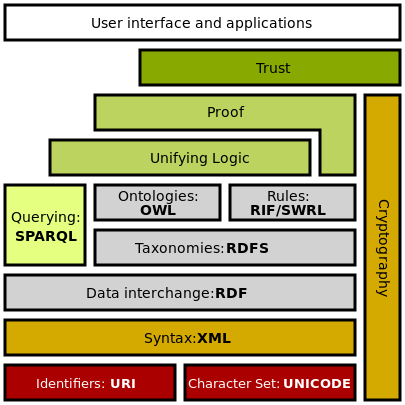
\includegraphics[width=.6\textwidth]{Semantic_web_stack.svg.png}}
\end{frame}

\begin{frame}
  \frametitle{Web Ontology Language (OWL)}
  \begin{itemize}
  \item OWL 2 is based on the Description Logic $\mathcal{SROIQ(D)}$
  \item $\mathcal{ALC}$ with
    \begin{itemize}
    \item complex role inclusions: $r \circ s \subseteq r$
    \item role hierarchy: $r \subseteq s$
    \item role transitivity $r \circ r \subseteq r$
    \item nominals: $\{ a_1,...,a_n\}$ as concept constructor
    \item qualified number restrictions: $(\leq n r.Q)$
    \item datatype properties: $\exists r.[\geq n (Integer)]$
    \end{itemize}
  \end{itemize}
\end{frame}

\begin{frame}
  \frametitle{OWL Reasoning}
  \begin{itemize}
  \item Classification: compute the most specific sub- and
    super-classes for each named class in an OWL ontology
  \item Subsumption: find all sub-, super- or equivalent classes of an
    OWL class description
  \item Consistency: find contradictions in DL knowledge base
  \item Instantiation: is $a$ and instance of $C$?
  \end{itemize}
\end{frame}

\begin{frame}
  \frametitle{Complexity of reasoning in OWL}
  \begin{itemize}
  \item OWL 2 ($\mathcal{SROIQ}$) is 2NEXPTIME-complete
  \item OWL (1) ($\mathcal{SHOIN}$) is NEXPTIME-complete
  \item OWL Lite ($\mathcal{SHIF}$) is EXPTIME-complete
  \end{itemize}
  \vspace{2cm}
\end{frame}

\begin{frame}
  \frametitle{OWL profiles}
  \begin{itemize}
  \item OWL 2 EL: PTIME-complete
  \item OWL 2 RL: PTIME-complete
  \item OWL 2 QL: $AC^0$ w.r.t. data size
  \end{itemize}
\end{frame}

\begin{frame}
  \frametitle{EL}
  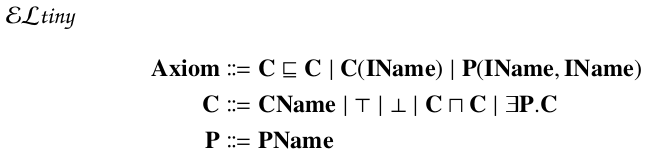
\includegraphics[width=0.8\textwidth]{eltiny.png}
  
\end{frame}

\begin{frame}
  \frametitle{RL}
  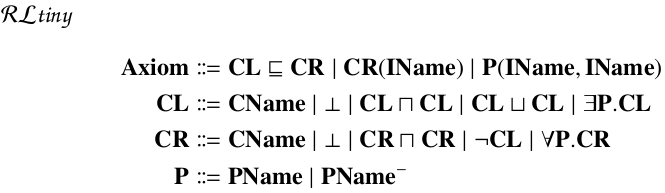
\includegraphics[width=0.8\textwidth]{rltiny.png}
  
\end{frame}

\begin{frame}
  \frametitle{QL}
  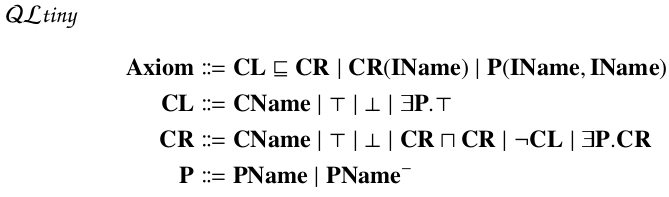
\includegraphics[width=0.8\textwidth]{qltiny.png}
  
\end{frame}

% \begin{frame}
%   \frametitle{Instance retrieval (ABox reasoning) in RL}
%   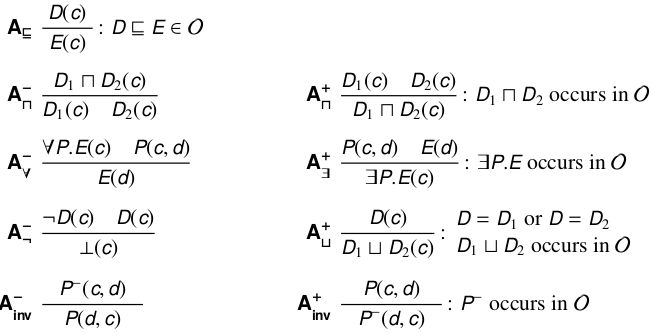
\includegraphics[width=0.8\textwidth]{rlrules.png}

% \end{frame}

% \begin{frame}
%   \frametitle{Instance retrieval in RL}
%   \begin{definition}[saturation]
%     An ontology is {\em saturated} under rules if it contains the
%     conclusions of all applicable rules. The {\em saturation} of an
%     ontology $O$ is the least saturated set $O'$ that contains $O$.
%   \end{definition}
%   \begin{itemize}
%   \item forward-chaining algorithm
%   \item computes the deductive closure
%   \end{itemize}
%   \begin{theorem}
%     The repeated application of the RL rules to an ontology $O$
%     terminates after at most $O(s^3)$ steps, where $s$ is the size of
%     $O$.
%   \end{theorem}

% \end{frame}

\begin{frame}
  \frametitle{Reasoning in EL}
  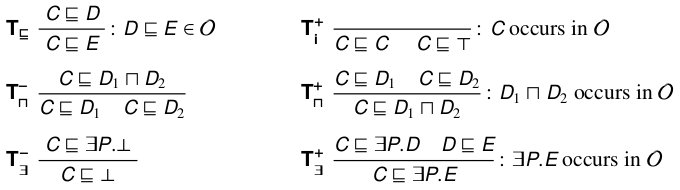
\includegraphics[width=0.8\textwidth]{elrules.png}
\end{frame}

\begin{frame}
  \frametitle{Sources of complexity}
  \begin{itemize}
  \item unions are hard -- non-deterministic
  \item universals + existentials = exponential
    \begin{itemize}
    \item proof using ATMs and reduction to QBFs
    \end{itemize}
  \item OWL EL + OWL QL = ExpTime
  \end{itemize}
\end{frame}

\begin{frame}
  \frametitle{Neuro-symbolic methods for DL}
  \begin{itemize}
  \item Use a FOL method like LTNs?
    \begin{itemize}
    \item for ABox reasoning?
    \item for TBox reasoning?
    \end{itemize}
    \pause
  \item Extending Knowledge Graph embeddings
    \begin{itemize}
    \item KGs are just ABox
    \item How to incorporate TBox and RBox?
    \end{itemize}
  \item Reasoning tasks
    \begin{itemize}
    \item Classification vs. subsumption
    \item explaining reasoning
    \end{itemize}
  \end{itemize}
\end{frame}

\begin{frame}
  \frametitle{Approaches for DL}
  \begin{itemize}
  \item graph-based (like knowledge graph embeddings)
  \item syntactic (like LNNs)
  \item geometric
  \end{itemize}
\end{frame}

\begin{frame}
  \frametitle{Graph}
  \begin{itemize}
  \item axiom patterns and graphs
  \end{itemize}
\end{frame}

\end{document}


%%% Local Variables:
%%% mode: latex
%%% TeX-master: t
%%% End:
